\documentclass[12pt]{article}

\usepackage[pdftex]{graphicx}
\usepackage{cancel}
\usepackage[margin=4cm]{geometry}
\usepackage[hidelinks]{hyperref}
\usepackage{fancyhdr}
\usepackage{amsmath}
\usepackage{amsfonts}
\usepackage{dirtytalk}

\newcommand\tab[1][1cm]{\hspace*{#1}}
\newcommand{\HRule}{\rule{\linewidth}{0.5mm}}
\newcommand{\course}{COMS 474}

\setcounter{secnumdepth}{0} % Disable section/subsection numbering
\hyphenpenalty 10000 % Prevent words from being broken over multiple lines
\exhyphenpenalty 10000 % Prevent words from being broken over multiple lines

% Margins
\topmargin=-0.45in
\evensidemargin=0in
\oddsidemargin=0in
\textwidth=6.5in
\textheight=9.0in
\headsep=0.25in
\title{ \course \\\large Homework 5 }
\author{ Haadi Majeed }
\date{Spring 2022}


\pagestyle{fancy}
\fancyhead{}
\fancyfoot{}
\lhead{\course}
\chead{Haadi Majeed}
\rhead{Page \thepage}

\begin{document}
\maketitle
\pagebreak

% Optional TOC
%\tableofcontents
\pagebreak
\section{Problem 1}
20 Points\\
Suppose you are predicting a feature $Y$ that can take on three values $Y \epsilon \{+1, +2, +3\}$ and you can predict $Y$ using two features $X_1$ and $X_2$. You decide to try LDA (i.e. we will estimate a different mean for each class but estimate a common covariance matrix). Suppose that the (common) covariance matrix you estimate is
\begin{center}
    $\sum_{+1} = \sum_{+2} = \sum_{+3} = \begin{bmatrix} 1 &0\\0 & 1\end{bmatrix}$
\end{center}
the priors are equal
\begin{center}
    $\pi_{+1} = \pi_{+2} = \pi_{+3} = \frac{1}{3}$
\end{center}
and the mean vectors are
\begin{center}
    $\mu_{+1} = \begin{bmatrix} -1\\-1\end{bmatrix}\tab\mu_{+2} = \begin{bmatrix} 1\\1\end{bmatrix}\tab\mu_{+3} = \begin{bmatrix} -1\\1\end{bmatrix}$
\end{center}

\subsection{A}
\subsubsection{Find the equation for the LDA boundry between $Y = +1$ and $Y = +2$}
Using figures 4.24 and figure 4.25 from the textbook\\
\begin{center}
    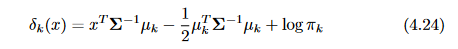
\includegraphics{fig4.24.png}\\
    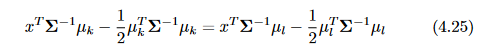
\includegraphics{fig4.25.png}
\end{center}
\[
    \delta_{+1}(x) = \delta_{+2}(x)
\]
\[
    x^T\begin{bmatrix} 1 & 0\\ 0 & 1\end{bmatrix}\begin{bmatrix} -1 \\ -1\end{bmatrix} - \frac{1}{2}\begin{bmatrix} -1 \\ -1\end{bmatrix}^T\begin{bmatrix} 1 & 0\\ 0 & 1\end{bmatrix}\begin{bmatrix} -1 \\ -1\end{bmatrix}
    =
    x^T\begin{bmatrix} 1 & 0\\ 0 & 1\end{bmatrix}\begin{bmatrix} 1 \\ 1\end{bmatrix} - \frac{1}{2}\begin{bmatrix} 1 \\ 1\end{bmatrix}^T\begin{bmatrix} 1 & 0\\ 0 & 1\end{bmatrix}\begin{bmatrix} 1 \\ 1\end{bmatrix}
\]
\[
    x^T\begin{bmatrix} -1 \\ -1\end{bmatrix}-\frac{1}{2}\begin{bmatrix}2\end{bmatrix}
    =
    x^T\begin{bmatrix} 1 \\ 1\end{bmatrix}-\frac{1}{2}\begin{bmatrix}2\end{bmatrix}
\]
\[
    \begin{bmatrix} x_1 \\ x_2\end{bmatrix}^T\begin{bmatrix} -1 \\ -1\end{bmatrix}-1
    =
    \begin{bmatrix} x_1 \\ x_2\end{bmatrix}^T\begin{bmatrix} 1 \\ 1\end{bmatrix} -1
\]
\[
    \begin{bmatrix} x_1 & x_2\end{bmatrix}\begin{bmatrix} -1 \\ -1\end{bmatrix}-1
    =
    \begin{bmatrix} x_1 & x_2\end{bmatrix}\begin{bmatrix} 1 \\ 1\end{bmatrix}-1
\]
\[
    \begin{bmatrix} -x_1 & -x_2\end{bmatrix}-1
    =
    \begin{bmatrix} x_1 & x_2\end{bmatrix}-1
\]
\[
    2\begin{bmatrix} x_1 & x_2\end{bmatrix} = 0
\]
\[
    \begin{bmatrix} x_1 & x_2\end{bmatrix} = 0
\]
\[
    x_1 + x_2 = 0
\]

\subsection{B}
\subsubsection{Find the equation for the LDA boundry between $Y = +1$ and $Y = +3$}
\[
    \delta_{+1}(x) = \delta_{+3}(x)
\]
\[
    x^T\begin{bmatrix} 1 & 0\\ 0 & 1\end{bmatrix}\begin{bmatrix} -1 \\ -1\end{bmatrix} - \frac{1}{2}\begin{bmatrix} -1 \\ -1\end{bmatrix}^T\begin{bmatrix} 1 & 0\\ 0 & 1\end{bmatrix}\begin{bmatrix} -1 \\ -1\end{bmatrix}
    =
    x^T\begin{bmatrix} 1 & 0\\ 0 & 1\end{bmatrix}\begin{bmatrix} -1 \\ 1\end{bmatrix} - \frac{1}{2}\begin{bmatrix} -1 \\ 1\end{bmatrix}^T\begin{bmatrix} 1 & 0\\ 0 & 1\end{bmatrix}\begin{bmatrix} -1 \\ 1\end{bmatrix}
\]
\[
    x^T\begin{bmatrix} -1 \\ -1\end{bmatrix}-\frac{1}{2}\begin{bmatrix}2\end{bmatrix}
    =
    x^T\begin{bmatrix} -1 \\ 1\end{bmatrix}-\frac{1}{2}\begin{bmatrix}2\end{bmatrix}
\]
\[
    \begin{bmatrix} x_1 \\ x_2\end{bmatrix}^T\begin{bmatrix} -1 \\ -1\end{bmatrix}-1
    =
    \begin{bmatrix} x_1 \\ x_2\end{bmatrix}^T\begin{bmatrix} -1 \\ 1\end{bmatrix} -1
\]
\[
    \begin{bmatrix} x_1 & x_2\end{bmatrix}\begin{bmatrix} -1 \\ -1\end{bmatrix}-1
    =
    \begin{bmatrix} x_1 & x_2\end{bmatrix}\begin{bmatrix} -1 \\ 1\end{bmatrix}-1
\]
\[
    \begin{bmatrix} -x_1 & -x_2\end{bmatrix}-1
    =
    \begin{bmatrix} -x_1 & x_2\end{bmatrix}-1
\]
\[
    2\begin{bmatrix} 0 & x_2\end{bmatrix} = 0
\]
\[
    \begin{bmatrix} 0 & x_2\end{bmatrix} = 0
\]
\[
    x_2 = 0
\]

\subsection{C}
\subsubsection{Find the equation for the LDA boundry between $Y = +2$ and $Y = +3$}

\[
    \delta_{+2}(x) = \delta_{+3}(x)
\]
\[
    x^T\begin{bmatrix} 1 & 0\\ 0 & 1\end{bmatrix}\begin{bmatrix} 1 \\ 1\end{bmatrix} - \frac{1}{2}\begin{bmatrix} 1 \\ 1\end{bmatrix}^T\begin{bmatrix} 1 & 0\\ 0 & 1\end{bmatrix}\begin{bmatrix} 1 \\ 1\end{bmatrix}
    =
    x^T\begin{bmatrix} 1 & 0\\ 0 & 1\end{bmatrix}\begin{bmatrix} -1 \\ 1\end{bmatrix} - \frac{1}{2}\begin{bmatrix} -1 \\ 1\end{bmatrix}^T\begin{bmatrix} 1 & 0\\ 0 & 1\end{bmatrix}\begin{bmatrix} -1 \\ 1\end{bmatrix}
\]
\[
    x^T\begin{bmatrix} 1 \\ 1\end{bmatrix}-\frac{1}{2}\begin{bmatrix}2\end{bmatrix}
    =
    x^T\begin{bmatrix} -1 \\ 1\end{bmatrix}-\frac{1}{2}\begin{bmatrix}2\end{bmatrix}
\]
\[
    \begin{bmatrix} x_1 \\ x_2\end{bmatrix}^T\begin{bmatrix} 1 \\ 1\end{bmatrix}-1
    =
    \begin{bmatrix} x_1 \\ x_2\end{bmatrix}^T\begin{bmatrix} -1 \\ 1\end{bmatrix} -1
\]
\[
    \begin{bmatrix} x_1 & x_2\end{bmatrix}\begin{bmatrix} 1 \\ 1\end{bmatrix}-1
    =
    \begin{bmatrix} x_1 & x_2\end{bmatrix}\begin{bmatrix} -1 \\ 1\end{bmatrix}-1
\]
\[
    \begin{bmatrix} x_1 & x_2\end{bmatrix}-1
    =
    \begin{bmatrix} -x_1 & x_2\end{bmatrix}-1
\]
\[
    -2\begin{bmatrix} x_1 & 0\end{bmatrix} = 0
\]
\[
    \begin{bmatrix} x_1 & 0\end{bmatrix} = 0
\]
\[
    x_1 = 0
\]

\subsection{D}
\subsubsection{Make a plot with $x_1$ along the horizontal axis, $x_2$ along the vertical axis and draw each of the LDA boundries you found. For each region, write the class label (e.g."+2") that would be chosen for a new sample that appeared in that region.}
\textbf{Note: the vertical axis is $x_2$ and the horizontal is $x_1$}
\begin{center}
    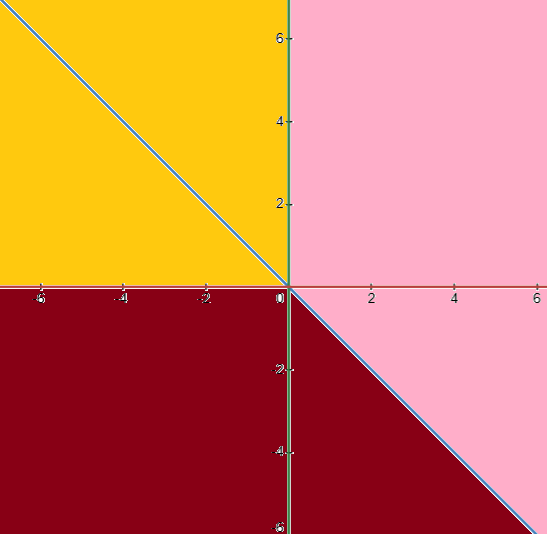
\includegraphics{p1.d.png}
\end{center}
With the Maroon representing $Y = +1$, Pink representing $Y = +2$, and the Yellow representing $Y= +3$.
With the following points being used to evaluate which had a greater value out of the trio:
\[\begin{matrix}
        x_1 & x_2 \\
        1   & 1   \\
        2   & -1  \\
        1   & -2  \\
        -2  & -2  \\
        -2  & 1   \\
        -1  & 2   \\
    \end{matrix}\]

\subsection{E}
\subsubsection{If you wanted to use Naive Bayes in addition to LDA (thus still assuming Gaussianity) for this problem explain what it would change (if anything)}
Bayes can be linear or curved, LDA can only be linear. If we were to use both and determine how the boundaries would change we could apply the fact the Bayes does not need independent covariance to the fact that LDA \emph{does} require it, therefore gaining the benefits of LDA's linear approach while lacking independent covariance from the set.



\pagebreak
\section{Problem 2}
15 Points\\
You intern for a university's athletics program and are tasked with predicting whether their rugby team will make it to the playoffs (Y $\epsilon$ \{yes, no\}) based on their  score in the first game of the season, X.\\\\
You collect data and estimate that for the years that the rugby team made it to the playoffs, their score in the first game had a mean of $\hat{\mu}_{yes} \approx 30$ and variance $\hat{\sigma}^2_{yes} \approx 50$. For the years that they did not make it to the playoffs, their score in the first game had a mean of $\hat{\mu}_{no} \approx 15$ and variance $\hat{\sigma}^2_{no} \approx 80$. The team made it to the playoffs $30\%$ of the years.\\\\
This year, they scored 20 points in their first game. Predict the probability that the team will make it to the playoffs. Use Bayes' theorem, and model the distribution of the first game scores, conditioned on whether or not they make it to the playoffs that year, as Gaussian.
\\\\
Bayes' Theorem: $\frac{\pi_kf_k(x)}{\sum^k_{l=1}\pi_lf_l(x)}$ or alternatively $P(A|B) = \frac{P(B|A)P(A)}{P(B)}$ With A resulting in Yes, they make it to the playoffs, and B resulting in No, they do not.

\[
    f_k(x) = \frac{1}{(2\pi)^{\frac{1}{2}}\sigma_k}^{-\frac{1}{2\sigma^2}(x-\mu_k)^2}
\]
\[
    p_k(x)=\frac{\pi_k\frac{1}{(2\pi)^{\frac{1}{2}}\sigma_k}^{-\frac{1}{2\sigma_k^2}(x-\mu_k)^2}}{\sum^k_{l=1}\pi_l\frac{1}{(2\pi)^{\frac{1}{2}}\sigma_l}^{-\frac{1}{2\sigma_l^2}(x-\mu_l)^2}}
\]

Additionally we have the following information from the problem:\\
\begin{center}
    \begin{tabular}{c c}
        $\pi_k = 0.3$       \tab$\pi_l = 0.7$   \\
        $\mu_k = 30$        \tab$\mu_l = 15$    \\
        $\sigma_k = 50$     \tab$\sigma_l = 80$ \\
    \end{tabular}
\end{center}

\[
    p_k(x)=\frac{0.3\frac{1}{(2*0.3)^{\frac{1}{2}}50}^{-\frac{1}{2*50^2}(x-30)^2}}{\sum^k_{l=1}0.7\frac{1}{(2*0.7)^{\frac{1}{2}}80}^{-\frac{1}{2*80^2}(x-15)^2}}
\]
\begin{center}
    after much math and a sad calculator (also with $x = 1$ and $k = 1$ since its just one game)...\\
    $p_k(x) = .7394$\\
    This results of a probability of about 73.94\% of making the playoffs from the information of the first game.
\end{center}
%--/Paper--

\end{document}